% vim:encoding=utf8 ft=tex sts=2 sw=2 et:

\documentclass{classrep}
\usepackage[utf8x]{inputenc}
\usepackage[a4paper, left=1.0cm, right=1.0cm, top=1.0cm, bottom=2.0cm, headsep=0.5cm, headheight=15pt]{geometry}
\usepackage{amsmath, amsthm, amssymb, amsfonts}
\usepackage{graphicx}
\usepackage{float}
\usepackage{listings}
\usepackage{hyperref} % musi być na końcu
\hypersetup{pdfborder={0 0 0 0}}


\studycycle{Elektronika i Telekomunikacja, studia dzienne, mgr II st.}
\coursesemester{II}

\coursename{Kompatybilność elektromagnetyczna }
\courseyear{2015/2016}

\courseteacher{dr inż. Wiesław Sabat}
\coursegroup{środa, 12:00}

\author{
  \studentinfo{Witold Olechowski}{127517} \and
  \studentinfo{Grzegorz Pelczar}{125242} \and
  \studentinfo{Mateusz Kut}{125212} \and
  \studentinfo{Tomasz Marecik}{127374} 
}

\title{Zadanie 6 : Badanie  odporności odkurzacza na znormalizowane rodzaje zaburzeń elektromagnetycznych. }



\begin{document}
\maketitle

\section{Cel ćwiczenia}

Badanie  odporności odkurzacza na znormalizowane rodzaje zaburzeń elektromagnetycznych tj. udar $1.2/50 \mu s$ zgodnie z zaleceniami standardu PN-EN 61000-4-5. Serię szybkich elektrycznych stanów przejściowych zgodnie z zaleceniami standardu PN-EN 61000-4-4 i zapady, krótkie przerwy i zmiany napięcia przejściowych, zgodnie z zaleceniami standardu PN-EN 61000-4-11

\section{Realizacja ćwiczenia}
Norma PN-EN 61000-4-5 określa wymagania odnośnie sprzętu, stanowiska pomiarowego oraz procedury badań odporności na udary napięciowe i prądowe. Parametry udarów również są ściśle określone. Ich poziomy pokazano na rysunku \ref{fig:wyk1}.

\begin{figure}[H]
\centering
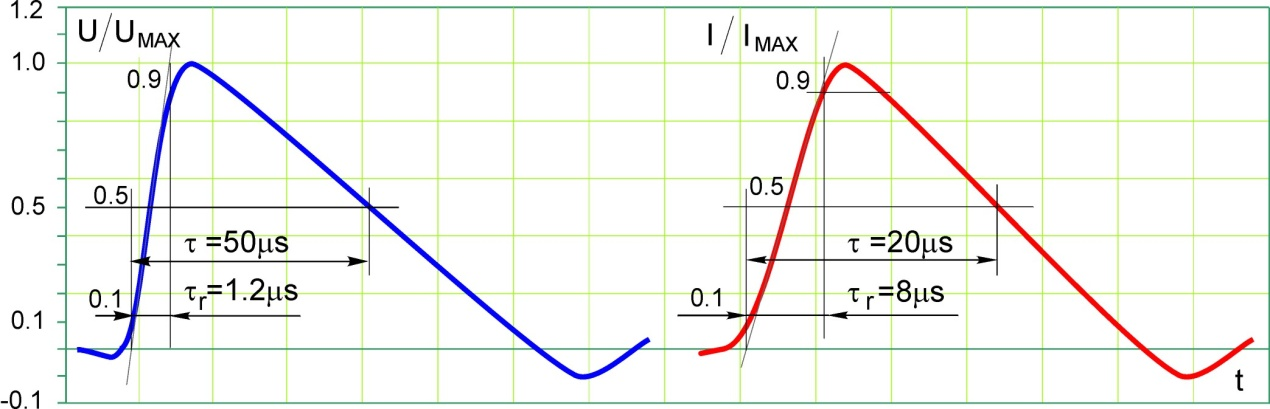
\includegraphics[width=0.7\linewidth]{wyk1}
\caption{Poziomy udarów.}
\label{fig:wyk1}
\end{figure}

W ramach wykonywanego ćwiczenia przeprowadzono test odporności odkurzacza na udar 1.2/50us. Wyniki przeprowadzonego testu zestawiono w tabeli.

\section{Zgodnie z zaleceniami standardu PN-EN 55014-2 pomiary przeprowadzić dla poziomu udaru 1kV, wstrzykiwanego pomiędzy przewód L-N, dla  chwil 0°, 90°, 180° i 270°.}

W ramach wykonywanego ćwiczenia przeprowadzono test odporności odkurzacza na udar 1.2/50us. Wyniki przeprowadzonego testu zestawiono w tabeli \ref{tab:1}.

\begin{table}[H]
	\centering
	\caption{Wyniki pomiaru odporności odkurzacza na udar $1.2/50 \mu s$.}
	\label{tab:1}
	\begin{tabular}{|l|l|l|l|l|}
		\hline
		\multicolumn{5}{|l|}{Udar $ 1.2/50 \mu s$, Up $-1kV$, Przewód L-N, $t_r =10s$, liczba udarów – 5, kryterium oceny B} \\ \hline
		\multicolumn{5}{|l|}{Warunki środowiskowe: Temperatura …… °C, Wilgotność wzgl. ….. \%.}                         \\ \hline
		L.p.         & Kąt          & Polaryzacja        & Wynik        & Ocena stanu pracy badanego urządzenia.        \\ \hline
		1.           & 0°           & +                  & +            & bez zastrzeżeń                                \\ \hline
		2.           & 90°          & +                  & +            & bez zastrzeżeń                                \\ \hline
		3.           & 180°         & +                  & +            & bez zastrzeżeń                                \\ \hline
		4.           & 270°         & +                  & +            & bez zastrzeżeń                                \\ \hline
		5.           & 0°           & -                  & +            & bez zastrzeżeń                                \\ \hline
		6.           & 90°          & -                  & +            & bez zastrzeżeń                                \\ \hline
		7.           & 180°         & -                  & +            & bez zastrzeżeń                                \\ \hline
		8.           & 270°         & -                  & +            & bez zastrzeżeń                                \\ \hline
		\end{tabular}
\end{table}
		

\section{Badania odporności na serię szybkich elektrycznych stanów przejściowych zgodnie z zaleceniami standardu PN-EN 61000-4-4.}


Badanie polega na sprawdzeniu wpływu na urządzenie zakłócenia w postaci serii 75 impulsów o amplitudzie 1kV. Serie są powtarzane co 300ms. Wyniki pomiaru odporności odkurzacza na serię szybkich elektrycznych stanów przejściowych przedstawiono w poniższej tabeli \ref{tab:2}.  Zgodnie z zaleceniami standardu PN-EN 55014-2 pomiary przeprowadzone dla poziomu udaru 1kV, wstrzykiwanego do przewodów L, N, L+N, dla  chwil 0°, 90°, 180° i 270°

\begin{table}[H]
	\centering
	\caption{Wyniki pomiaru odporności odkurzacza na serię szybkich elektrycznych stanów przejściowych}
	\label{tab:2}
	\begin{tabular}{|l|l|l|l|l|}
		\hline
		\multicolumn{5}{|l|}{\textbf{\begin{tabular}[c]{@{}l@{}}Impuls 5/50ns, N – 75 imp, f – 5kHz, tp=15ms, tr =300ms,  Up -1kV,\\  Przewód: L, N, L+N, czas narażenia – 1min, kryterium oceny  B\end{tabular}}} \\ \hline
		\multicolumn{5}{|l|}{\textbf{Warunki środowiskowe: Temperatura …… °C, Wilgotność wzgl. ….. \%.}}                                                                                                           \\ \hline
		L.p.                         & Kąt                               & Polaryzacja                         & Wynik                             & Ocena stanu pracy badanego urządzenia.                        \\ \hline
		1.                           & L 0°                              & +/-                                 & \textbf{+}                        & \textbf{bez zastrzeżeń}                                       \\ \hline
		2.                           & L 90°                             & +                                   & \textbf{+}                        & \textbf{bez zastrzeżeń}                                       \\ \hline
		3.                           & L 180°                            & +                                   & \textbf{+}                        & \textbf{bez zastrzeżeń}                                       \\ \hline
		4.                           & L 270°                            & +                                   & \textbf{+}                        & \textbf{bez zastrzeżeń}                                       \\ \hline
		5.                           & N 0°                              & +/-                                 & \textbf{+}                        & \textbf{bez zastrzeżeń}                                       \\ \hline
		6.                           & N 90°                             & +                                   & \textbf{+}                        & \textbf{bez zastrzeżeń}                                       \\ \hline
		7.                           & N180°                             & +                                   & \textbf{+}                        & \textbf{bez zastrzeżeń}                                       \\ \hline
		8.                           & N 270°                            & +                                   & \textbf{+}                        & \textbf{bez zastrzeżeń}                                       \\ \hline
		9.                           & L+N 0°                            & +/-                                 & \textbf{+}                        & \textbf{bez zastrzeżeń}                                       \\ \hline
		10.                          & L+N 90°                           & +                                   & \textbf{+}                        & \textbf{bez zastrzeżeń}                                       \\ \hline
		11.                          & L+N 180°                          & +                                   & \textbf{+}                        & \textbf{bez zastrzeżeń}                                       \\ \hline
		12.                          & L+ N 270°                         & +                                   & \textbf{+}                        & \textbf{bez zastrzeżeń}                                       \\ \hline
	\end{tabular}
\end{table}

\section{Badania odporności na zapady i zaniki  napięcia. Zgodnie z zaleceniami standardu PN-EN 55014-2.}

Ostatnim zadaniem było zbadanie odporności odkurzacza na zapady i zaniki napięcia. rządzenie może się wyłączył w wyniku zapadu napięcia, ale po zniknięciu zakłóceń musi wrócić do pracy w trybie, w którym było ustawione, bądź do trybu określonego przez producenta.

\begin{table}[H]
	\centering
	\caption{Wyniki pomiaru odporności odkurzacza na zapady i zaniki napięcia zasilania}
	\label{tab:3}
	\begin{tabular}{|l|l|l|l|l|}
		\hline
		\multicolumn{5}{|l|}{\textbf{Warunki środowiskowe: Temperatura 24 °C, Wilgotność wzgl. 80 \%.  Kryterium oceny C}} \\ \hline
		L.p.       & Kąt              & Czas trwania       & Wynik            & Ocena stanu pracy badanego urządzenia.      \\ \hline
		1.         & Zapad  40°       & 10 x 20ms          & \textbf{+}       & \textbf{bez zastrzeżeń}                     \\ \hline
		2.         & Zapad  70°       & 50 x 20ms          & \textbf{+}       & \textbf{bez zastrzeżeń}                     \\ \hline
		3.         & Zanik  100°          & 0.5 x 20ms         & \textbf{+}       & \textbf{bez zastrzeżeń}                     \\ \hline
	\end{tabular}
\end{table}

\section{Wnioski}
W ramach wykonywanego ćwiczenia zapoznano się z normami określającymi metody badania odporności urządzeń na różnego rodzaju zakłócenia elektryczne. Zgodnie z tymi regułami przeprowadzono sprawdzono odporność odkurzacza na udar 1.2/50, serię szybkich elektrycznych stanów przejściowych oraz zapady i zaniki napięcia.
Na podstawie przeprowadzonych testów należy stwierdzić, że badany odkurzacz został odpowiednio zabezpieczony przed zakłóceniami.

\begin{thebibliography}{0}
	\bibitem{l2short}  Wiesław Sabat,
	\textsl{Instrukcje laboratoryjne,} Politechnika Rzeszowska, Rzeszów, 2015
\end{thebibliography}
\end{document}
